\chapter{Hidrocarbonetos}
\begin{mdframed}[backgroundcolor=orange!20,linewidth=0pt,roundcorner=10pt]
	\minitoc
\end{mdframed}
Os hidrocarbonetos são uma classe fundamental de compostos químicos que desempenham um papel central na química orgânica. Eles consistem exclusivamente em átomos de carbono e hidrogênio, formando uma família diversificada de moléculas que variam desde as mais simples até as mais complexas. A simplicidade de sua composição, que consiste apenas em dois elementos, torna os hidrocarbonetos um dos grupos de compostos mais estudados e essenciais na química orgânica, e um exemplo destes pode ser visto na figura \ref{fig:ocatene}

\begin{figure}[h]\centering
\caption{Um hidrocarboneto encontrado no petróleo}
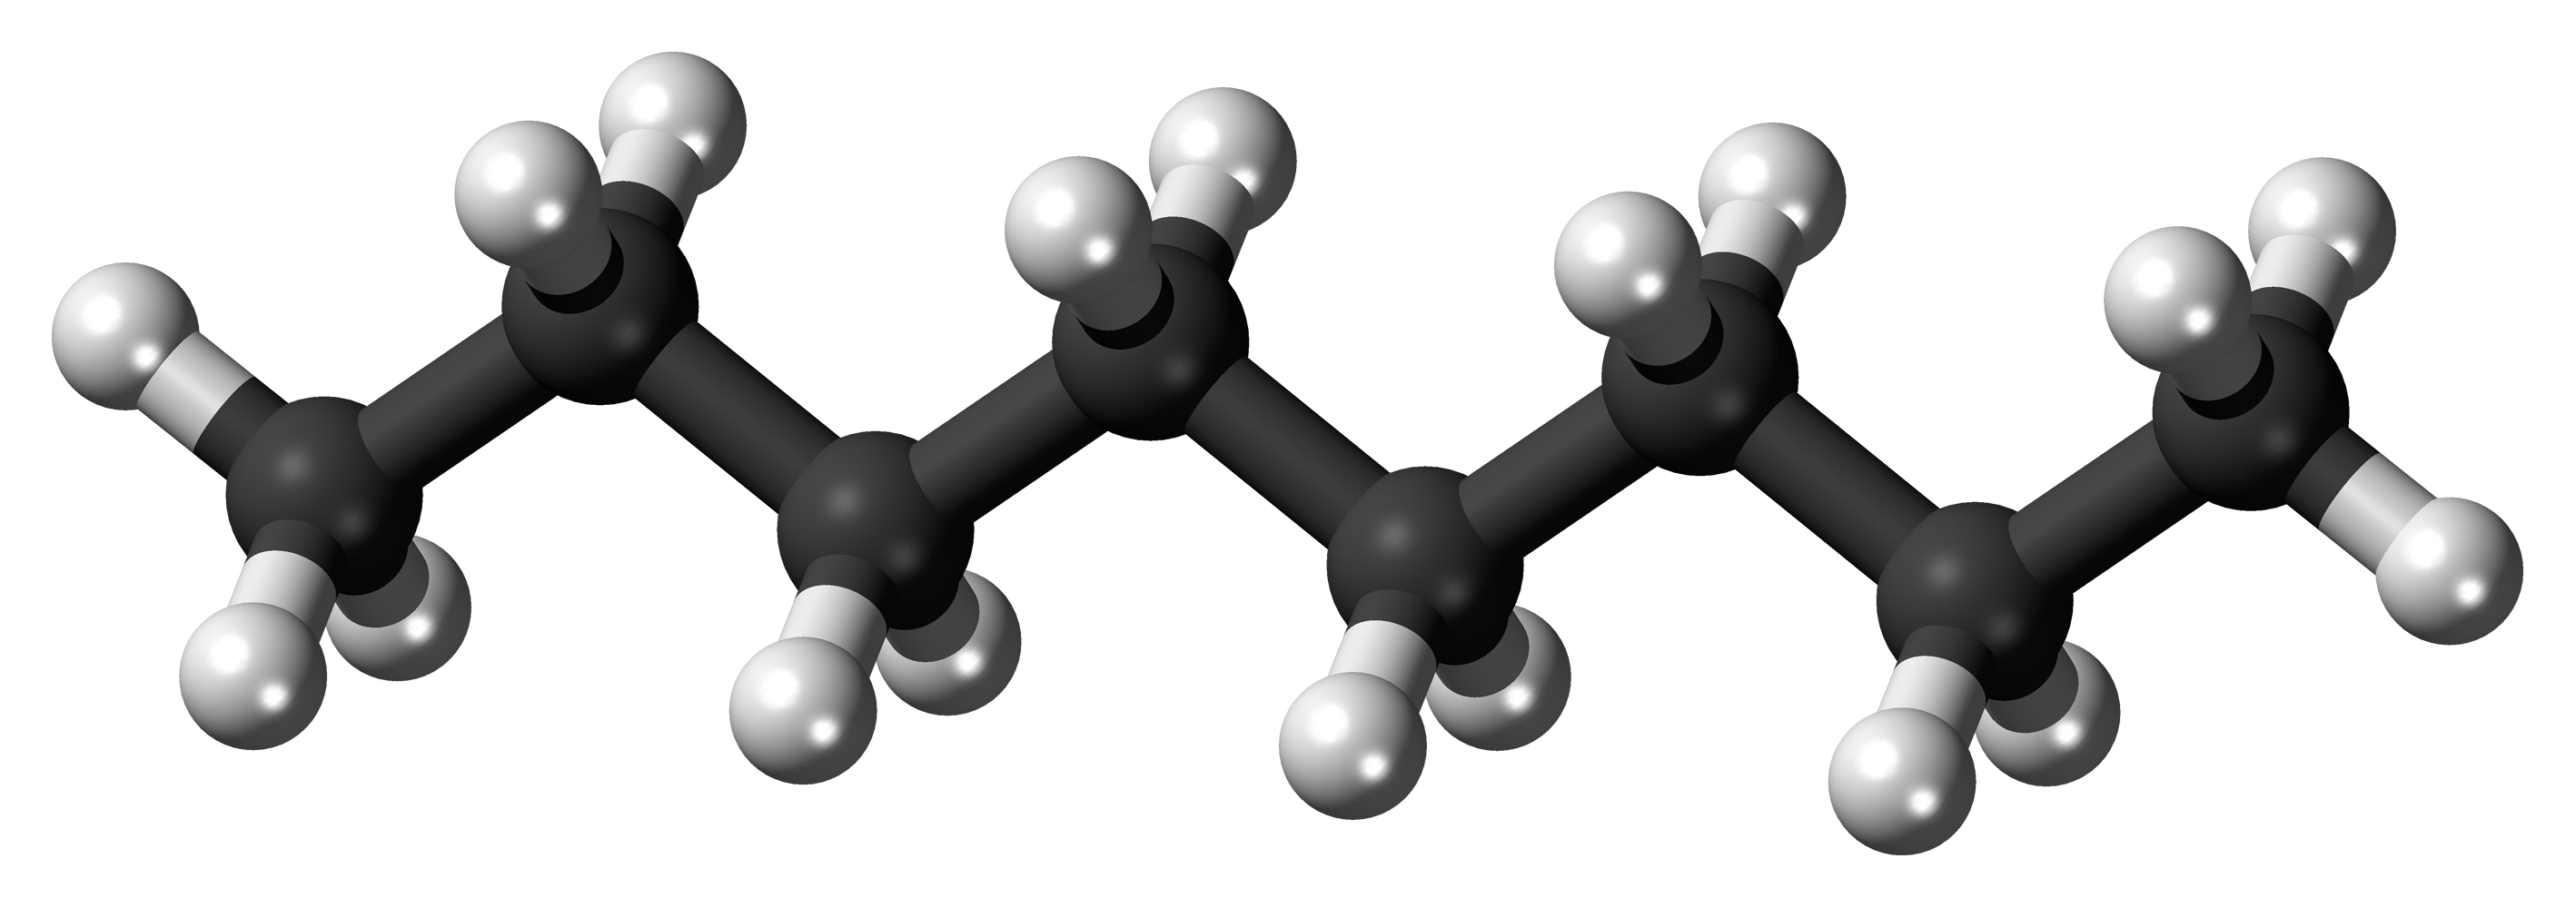
\includegraphics[scale=0.175]{imagens/Octane_3D_ball.png}
\label{fig:ocatene}\vspace{0.5cm}\end{figure}

Algumas das características da representação estrutural presente na figura \ref{fig:ocatene} serão úteis em diversos outros momentos deste livro e podemos tratar rapidamente sobre algumas delas. Repare que a figura apresenta tubos (para representar ligações covalentes) e esferas (para representar átomos). Os átomos mais claros são Hidrogênio e os mais escuros são Carbono. Um único tubo entre dois átomos representa uma \textbf{ligação covalente simples}, dois tubos representam uma \textbf{ligação covalente dupla} (ausente na figura) e três tubos representam a \textbf{ligação covalente tripla} (também ausente na figura).

Ainda na figura \ref{fig:ocatene}, todos os átomos de carbono encontram-se ligados por ligações covalentes simples, o que classifica essa sequência de átomos de carbono, a partir deste ponto chamada de \textbf{cadeia carbônica} como \textbf{cadeia saturada}. Caso a cadeia carbônica possua uma ligação covalente dupla entre o carbono da extremidade esquerda e seu vizinho imediato (neste exemplo), conforme pode ser visto na figura \ref{fig:hexene}, a cadeia passa a ser classificada como insaturada.

\begin{figure}[h]\centering
\caption{Um hidrocarboneto insaturado}
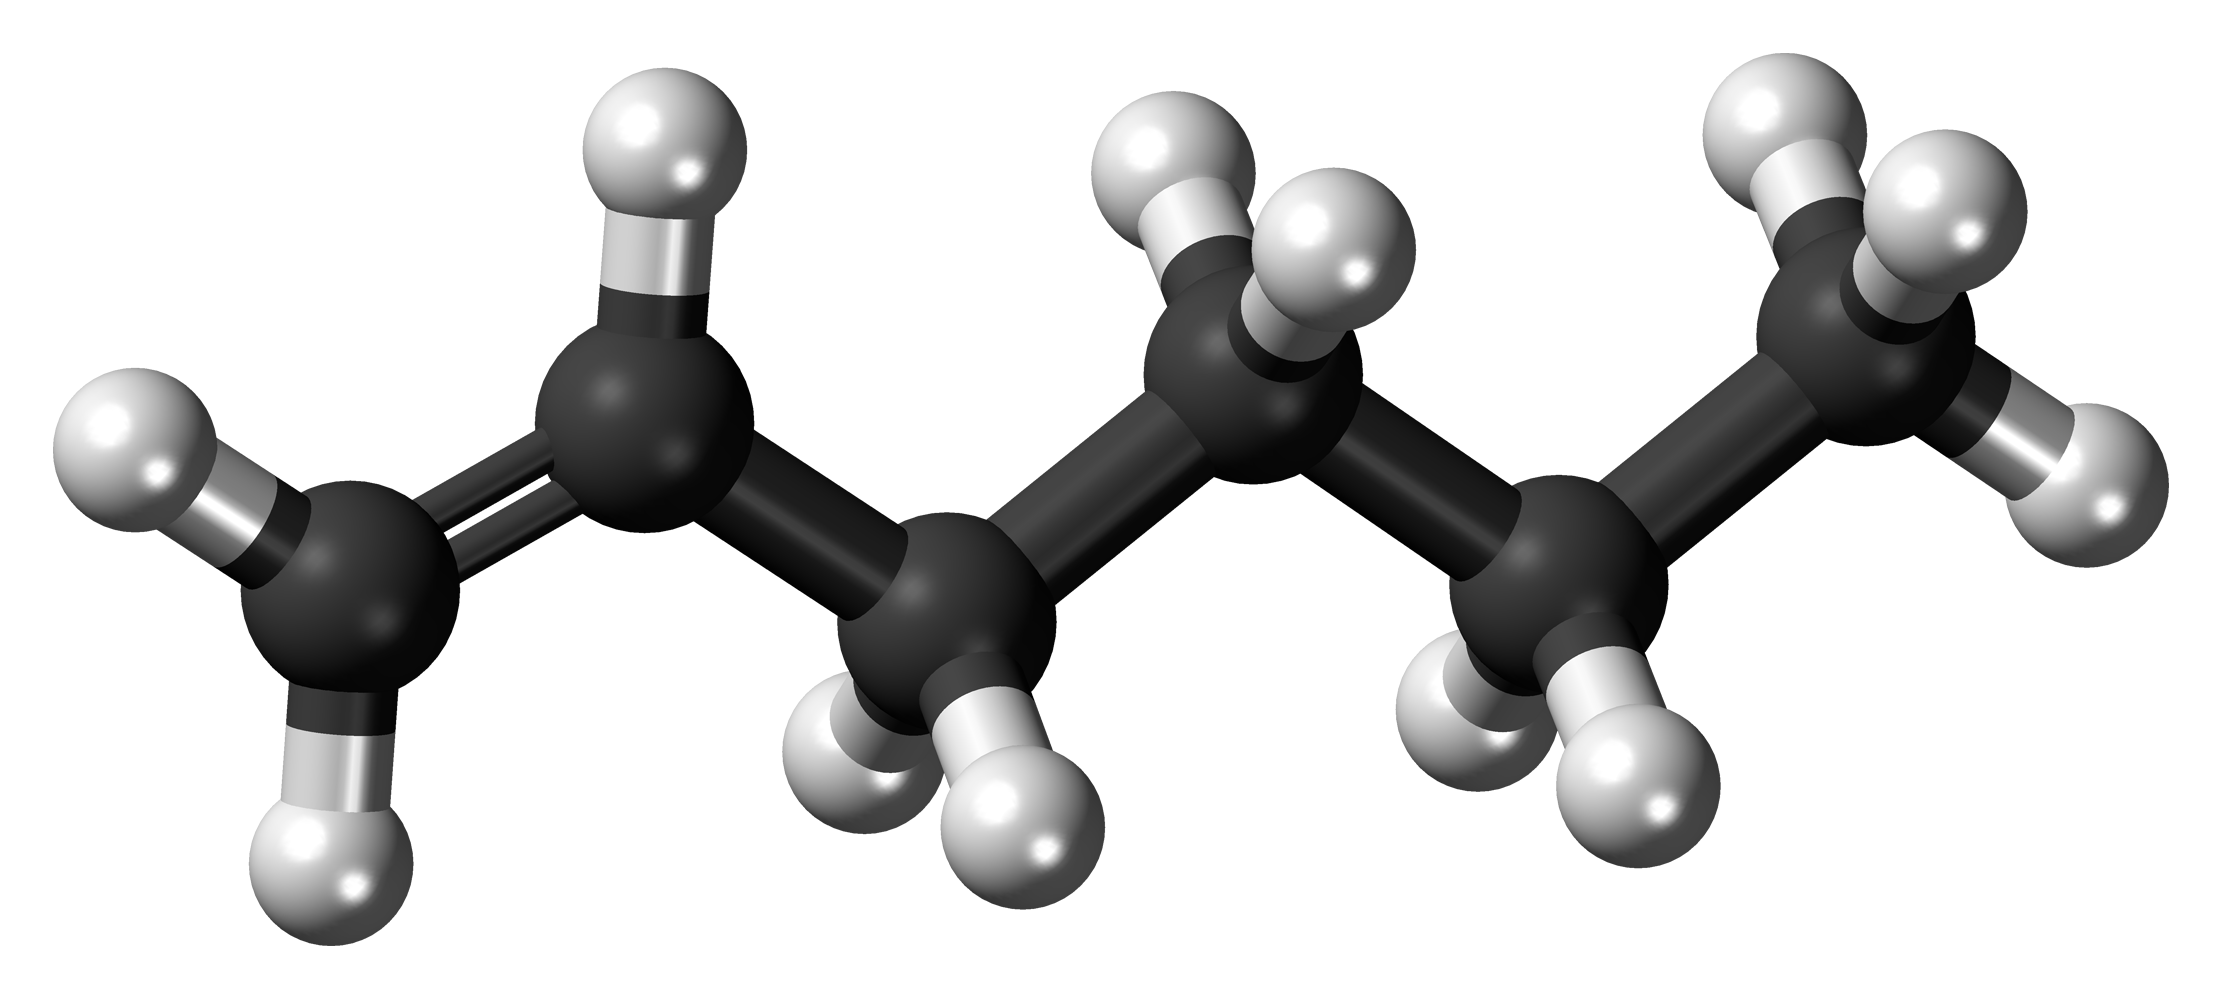
\includegraphics[scale=0.225]{imagens/1-Hexene-3D-balls.png}
\label{fig:hexene}\vspace{0.5cm}\end{figure}

Os hidrocarbonetos desempenham um papel vital em inúmeros aspectos da nossa vida cotidiana. Eles são os principais constituintes dos combustíveis fósseis, como petróleo e gás natural, que propulsionam nossos veículos e fornecem energia para a geração de eletricidade. Além disso, muitos produtos químicos, plásticos e materiais sintéticos são derivados de hidrocarbonetos.

Esta introdução explorará a estrutura básica dos hidrocarbonetos, suas diferentes categorias e sua relevância em várias aplicações, desde o setor energético até a indústria química e farmacêutica, destacando sua importância na química orgânica e na nossa sociedade moderna.
\section{Origens do petróleo}
A teoria orgânica para a origem do petróleo é uma das explicações mais aceitas para a formação desse recurso natural. Ela postula que o petróleo se origina a partir da decomposição de matéria orgânica, como plantas e microorganismos, ao longo de milhões de anos sob condições específicas de pressão e temperatura no subsolo. Esta teoria foi proposta pela primeira vez no século XIX e é conhecida como a teoria biogênica.

A \textbf{teoria orgânica} descreve o processo de formação do petróleo da seguinte maneira:

1. Acúmulo de Matéria Orgânica: No passado geológico, oceanos e lagos continham uma grande quantidade de matéria orgânica em diferetnes estados de decomposição, incluindo plâncton, algas e outros resíduos biológicos. Toda essa matéria orgânica se acumulava no fundo dessas águas, onde a falta de oxigênio limitava a decomposição completa.

2. Sepultamento: Com o tempo, sedimentos foram se acumulando sobre a matéria orgânica, causando seu sepultamento no subsolo. Essa incrível sobreposição de sedimentos exerceu pressão sobre a matéria orgânica, comprimindo-a.

3. Aumento de Temperatura e Pressão: À medida que os sedimentos continuaram a se acumular, a temperatura e a pressão no subsolo aumentaram gradualmente. A essa profundidade, a matéria orgânica passou por uma série de transformações químicas conhecidas como diagênese. Durante esse processo, a matéria orgânica se transformou em uma mistura complexa de hidrocarbonetos.

4. Migração e Armazenamento: Os hidrocarbonetos resultantes do processo de diagênese migraram através de rochas porosas e segmentos impermeáveis em direção às camadas superiores. Eles eventualmente ficaram presos em bolsas subterrâneas, formando reservatórios de petróleo.

5. Processo de Maturação: Com o tempo, os hidrocarbonetos continuaram a sofrer mudanças químicas, refinando-se e produzindo petróleo bruto, gás natural e outros componentes. A qualidade e a composição do petróleo podem variar dependendo das condições geológicas locais.

É importante observar que a teoria orgânica não é a única explicação para a origem do petróleo. Existem outras teorias, como a teoria abiótica, que sugere que o petróleo pode ser formado a partir de processos químicos não relacionados à matéria orgânica. No entanto, a teoria orgânica é amplamente aceita e tem uma base sólida na geologia e na química orgânica. Ela também se alinha com a grande quantidade de evidências geológicas e experimentais coletadas ao longo de muitas décadas.

A teoria inorgânica para a origem do petróleo é uma explicação alternativa à teoria orgânica predominante. Enquanto a teoria orgânica postula que o petróleo se forma a partir da decomposição de matéria orgânica, como microorganismos marinhos e plantas terrestres, a teoria inorgânica sugere que o petróleo pode se originar de processos não relacionados a organismos vivos.

A \textbf{teoria inorgânica} propõe que o petróleo é formado por reações químicas no interior da Terra, envolvendo elementos inorgânicos, como carbono, hidrogênio e nitrogênio. Os defensores dessa teoria argumentam que o petróleo é encontrado em profundidades muito maiores do que seria esperado se fosse proveniente de restos orgânicos, e que os processos geológicos e químicos subterrâneos podem produzir hidrocarbonetos a partir de substâncias não orgânicas.

Uma das principais hipóteses dentro da teoria inorgânica é a abiotica, que sugere que o petróleo é produzido por reações químicas de alta pressão e temperatura no manto da Terra, muito abaixo da camada onde a matéria orgânica é encontrada. Essas reações envolvem a transformação de minerais ricos em carbono, como calcário e magnésio, em hidrocarbonetos.

No entanto, é importante destacar que a teoria inorgânica enfrenta desafios significativos e não é amplamente aceita na comunidade científica. A teoria orgânica tem uma base sólida de evidências geológicas, juntamente com evidências geoquímicas e paleontológicas que apoiam a origem orgânica do petróleo. Além disso, a teoria inorgânica ainda não conseguiu explicar completamente a diversidade de compostos encontrados no petróleo cru.

\section{Classificação}
A classificação de hidrocarbonetos é um tópico fundamental na química orgânica, uma vez que os hidrocarbonetos constituem a base de muitos compostos orgânicos. Os hidrocarbonetos são compostos formados exclusivamente por átomos de carbono (C) e hidrogênio (H) e podem ser categorizados de acordo com a natureza das ligações entre os átomos de carbono e sua estrutura geral. Existem três grandes  categorias principais de hidrocarbonetos: alcanos, alcenos e alcinos, cada uma com características distintas.

1. \textbf{Alcanos}: são hidrocarbonetos que possuem apenas em ligações simples (ligações sigma) entre os átomos de carbono. Eles são conhecidos como hidrocarbonetos saturados, pois apresentam a máxima quantidade possível de hidrogênios. A fórmula geral dos alcanos é CnH2n+2, onde "n" representa o número de átomos de carbono na cadeia. Exemplos de alcanos incluem o metano (\ce{CH4}), o etano (\ce{C2H6}), o propano (\ce{C3H8}) e o butano (\ce{C4H10}). Alcanos têm pontos de ebulição mais baixos e são geralmente menos reativos em comparação com outras classes de hidrocarbonetos.

\begin{figure}[h]\centering
\caption{Um exemplo de hidrocarboneto do tipo alcano, com fórmula molecular \ce{C8H18}}
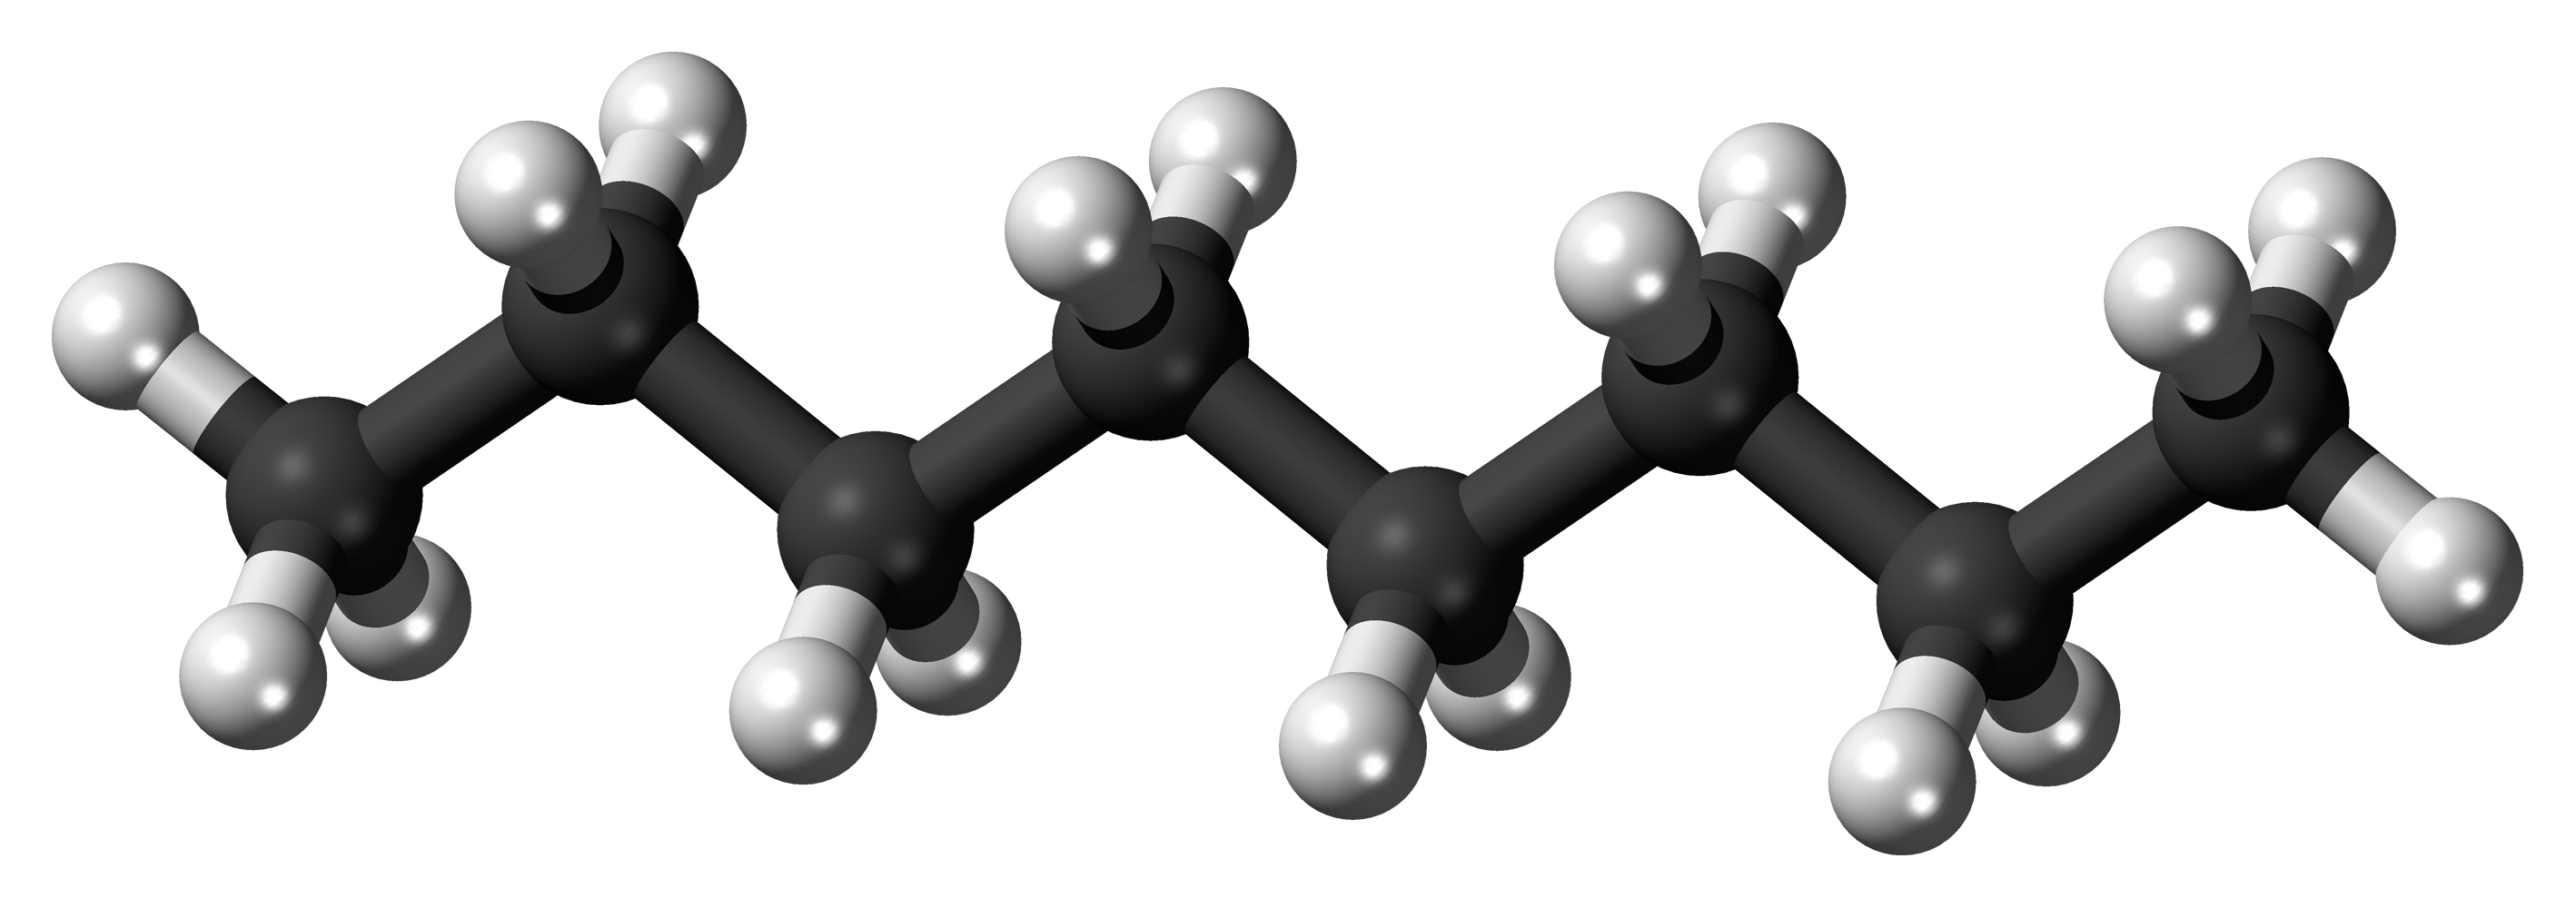
\includegraphics[scale=0.15]{imagens/Octane_3D_ball.png}
\label{fig:alcano}\vspace{0.5cm}\end{figure}

2. \textbf{Alcenos}:
Os alcenos são hidrocarbonetos que contêm pelo menos uma ligação dupla (ligação pi) entre átomos de carbono na cadeia. A fórmula geral dos alcenos é CnH2n, onde "n" representa o número de átomos de carbono na cadeia. A presença da ligação dupla introduz uma insaturação na molécula. Exemplos de alcenos incluem o eteno (\ce{C2H4}), o propeno (\ce{C3H6}) e o buteno (\ce{C4H8}). Os alcenos tendem a ser mais reativos do que os alcanos devido à presença da ligação dupla, que permite a ocorrência de reações de adição.

3. \textbf{Alcinos}:
Os alcinos são hidrocarbonetos que contêm pelo menos uma ligação tripla (duas ligações pi e uma ligação sigma) entre átomos de carbono na cadeia. A fórmula geral dos alcinos é CnH2n-2, onde "n" representa o número de átomos de carbono na cadeia. A ligação tripla torna os alcinos ainda mais reativos do que os alcenos e alcanos. Exemplos de alcinos incluem o etino (C2H2) e o propino (C3H4). Devido à sua alta reatividade, os alcinos são frequentemente usados como intermediários em sínteses orgânicas.

Além dessa classificação básica, os hidrocarbonetos também podem ser classificados com base na sua estrutura ramificada ou cíclica:

1. \textbf{Ramificados}:

Hidrocarbonetos podem apresentar grupos alquilas, também ligados à cadeia principal. A presença de destas leva à formação de isômeros, que são compostos com a mesma fórmula molecular, mas com diferentes arranjos espaciais. Os isômeros podem ter propriedades químicas e físicas distintas.

\begin{figure}[h]\centering
\caption{Um exemplo de hidrocarboneto ramificado}
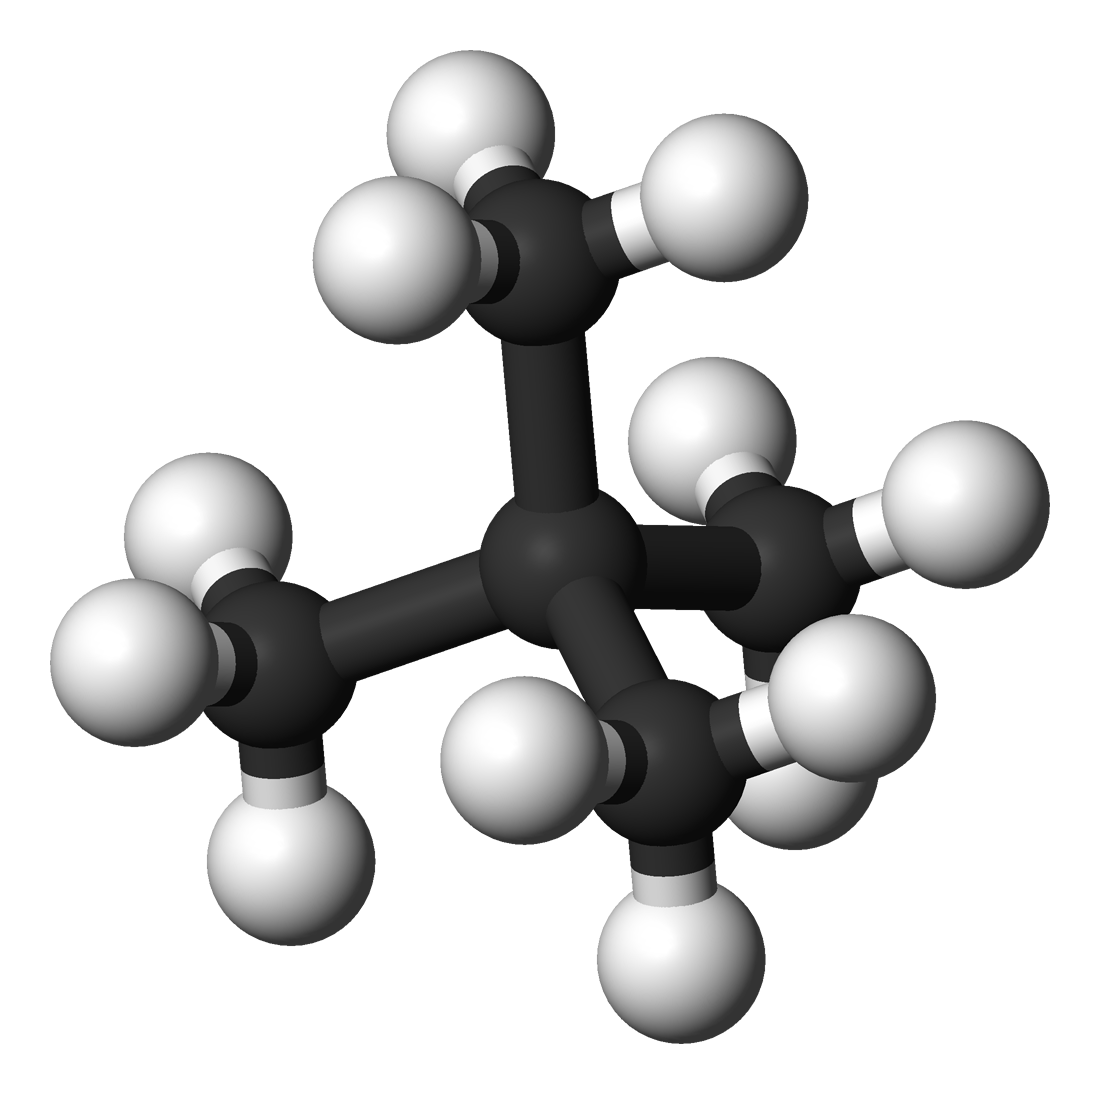
\includegraphics[scale=0.125]{imagens/Neopentane-3D-balls.png}
\label{fig:ramificado}\vspace{0.5cm}\end{figure}

2. \textbf{Cíclicos}:

Muitos hidrocarbonetos formam anéis fechados em suas estruturas. Esses compostos são chamados de hidrocarbonetos cíclicos. O ciclo mais simples é o ciclopropano, composto por um anel de três carbonos. Cicloexano, ciclopentano e ciclobutano são outros exemplos de hidrocarbonetos cíclicos.

\begin{figure}[h]\centering
\caption{Representação do cicloexano na notação \textbf{bastão}}

\includegraphics[scale=0.1]{imagens/2560px-Chair_conformation_of_cyclohexane.svg.png}
\label{fig:cicloexano}\vspace{0.5cm}\end{figure}

A figura \ref{fig:cicloexano} apresenta um dos mais belos e complexos temas da Química Orgânica: os fundamentos da análise conformacional. Analisar a forma tridimensional de uma molécula é fundamental para compreender sua interação com outras moléculas ou então com substratos biológicos. Em tal representação, as ligações Carbono-Hidrogênio são omitidas por clareza e as ligações Carbono-Carbono são representadas por um traço. Na figura vemos traços mais grossos que outro, usados aqui para fornecer uma ideia tridimensional em um veículo nitidamente bidimensional, este livro. Assuma quem, quando um traço estiver mais grosso, os átomos envolvidos estão espacialmente mais próximos do leitor do que os demais.

Além dessas categorias, a aromaticidade é uma propriedade especial observada em alguns hidrocarbonetos, como o benzeno. Moléculas consideradas aromáticas apresentam uma estabilidade excepcional devido ao fenômeno conhecido por ressonância eletrônica em seu sistema de anel, tornando-as distintas das categorias mencionadas anteriormente.

A classificação de hidrocarbonetos é essencial na química orgânica, pois ajuda os químicos a compreenderem a estrutura, as propriedades e o comportamento desses compostos. Além disso, a capacidade de categorizar os hidrocarbonetos facilita a previsão de suas reações químicas e aplicações em diversas áreas, como indústria, farmácia e pesquisa científica. 

\section{Estrutura}
A representação estrutural de um hidrocarboneto, assim como nos demais compostos orgânicos, pode ser feita de diferentes formas, dependendo da finalidade ou necessidade específica. Como exemplo, podemos nos deparar com uma publicação científica que exige a representação de uma molécula com uso de pouco espaço, onde o foco não deve ser apenas na estrutura, mas no contexto global, como pôsteres em congressos.

As mais comuns representações moleculares em Química Orgânica são as seguintes:
\begin{itemize}
\item Fórmula estrutural completa
\item Fórmula estrutural condensada
\item Fórmula estrutural em bastão
\item Fórmula estrutural com preenchimento espacial
\end{itemize}

\section{Propriedades físicas de hidrocarbonetos}
Hidrocarbonetos são substâncias formadas apenas por átomos e carbono e átomos de hidrogênio, constituindo a espinha dorsal que pode originar muitas moléculas encontradas na natureza. Podem ser classificados em várias categorias, e suas propriedades físicas são importantes para compreender suas reações em condições naturais e industriais.

\subsection{Pontos de Fusão e Ebulição}

Os pontos de fusão dos hidrocarbonetos são afetados preferencialmente pelo número de átomos de carbono em suas moléculas e pelo arranjo topológico e espacial entre esses átomos. Os hidrocarbonetos classificados como saturados, como os alcanos, tendem a apresentar pontos de ebulição mais baixos, enquanto alcenos e alcinos (insaturados com ligação dupla ou tripla, respectivamente) tendem a apresentar pontos de ebulição mais elevados. A razão do auimento nos valores de PF é simples: sendo apolares, as moléculas dos hidrocabonetos atraem-se por meio das chamadas Forças de London, tipicamente fracas, mas à medida em que o número de átomos de carbono aumenta, tal atração torna-se acumulativamente mais significante e, portanto, os valores de PF aumentam. Veja um exemplo na tabela \ref*{pf} a seguir.

\begin{table}[!h]
\begin{center}
\caption{\label{pf}Temperaturas de fusão e ebulição de alguns hidrocarbonetos saturados.}
\vspace{0.5cm}
\begin{tabular}{|c|c|c|c|c|}
\hline
Substância & Fórmula & Massa molar (g/mol) & TF ({$^o$}C) & TE ({$^o$}C)\\
\hline
Metano & \ce{CH4} & 16 & -182 & -161 \\
\hline
Etano & \ce{C2H6} & 30 & -183 & -87 \\
\hline
Propano & \ce{C3H8} & 44 & -188 & -42 \\
\hline
Butano & \ce{C4H10} & 58 & -138 & -0,5 \\
\hline
Pentano & \ce{C5H12} & 72 & -130 & -36 \\
\hline
\end{tabular}
\end{center}
\end{table}

Os pontos de ebuilição dos hidrocarbonetos estão intimamente relacionados com o tamanho e a forma das moléculas. Por tal razão, dois hidrocarbonetos isômeros de cadeia (moléculas com mesma fórmula molecular, mas com cadeias carbônicas distintas), pentano e 2,2-dimetil-propano possuem Ponto de Ebulição tão distintos. A cadeia carbônica do pentano é normal (sem ramificações), enquanto a cadeia carbônica do 2,2-dimetil-propano é ramificada, o a faz tender a um formato esférico, com menor área superficial que o pentano. Assim, as forças de atração no poentano se tornam maiores e os PF são tão distintos, conforme pode ser visto na figura \ref{fig:pentano} a seguir.

\begin{figure}[H]
	\centering
	\caption{Influência da forma da molécula nos valore de PE}
	\vspace{0.5cm}
	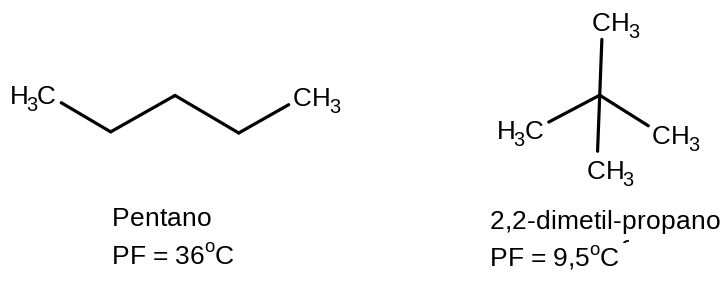
\includegraphics[width=1\linewidth]{imagens/pentano_22dimetil.png}
\label{fig:pentano}
\end{figure}


\subsection{Solubilidade}

A solubilidade dos hidrocarbonetos em água é geralmente muito baixa devido à natureza apolar de suas moléculas. No entanto, a solubilidade pode aumentar ligeiramente com o tamanho da cadeia crbônica, pois moléculas maiores possuem área superficial maior para interagir com as moléculas de água, mas isso só ocorre em poucas situações, como emulsões ou então quando óleo (mistura complexa de hidrocarbonetos) flutua na água.

A solubilidade é uma característica importante para a separação de hidrocarbonetos em processos de refino de petróleo e na indústria química. Sendo moléculas apolares, os hidrocarbonetos tendem a dissolver-se em moléculas igualmente apolares e, portanto, tendem a não interagir com água. Porém, dissolvem-se bem em solventes igualmente apolares, como benzeno (\ce{C6H6}).

De modo geral, hidrocarbonetos de cadeias curtas são mais solúveis em solventes apolares do que hidrocarbonetos de cadeia carbônica maior, pois moléculas menores podem dispersar-se melhor entre as moléculas do solvente. A ramificação das cadeias carbônicas dos hidrocarbonetos pode aumntar sua solubilidade em solventes apolares, uma vez que a área superficial é reduzida e uma molécula compacta dispersa-se melhor que uma molécula maior.

 

\subsection{Densidade}
A densidade de hidrocarbonetos varia com sua composiçao e estrutura molecular. Normalmente, os HC mais leves, como metano (\ce{C4}) ou etano (\ce{C2H6}) saõ menos densos que o ar, são inflamáveis e tendem a ascender, uma vez que todo gás menos denso que o ar sofre esse fenônemo. A densidade é uma característica  importante em processos de separação, como a destilação, através da qual os componentes são separados com base em suas diferenças de densidade. De modo geral, quanto maior a massa molar de um hidrocarboneto, maior será sua densidade, uma vez que uma molécula mais pesada apresenta maior massa por unidade de volume. Como exemplo, o propano (\ce{C3H8}) apresenta densidade com valor \textbf{0,498 g/mL} enquanto o decano (\ce{C10H22}) apresenta densidade com valor \textbf{0,730 g/mL} na mesma temperatura de 20{$^o$}C.

\subsection{Tensão Superficial}
Em uma amostra de água, existem dois tipos de moléculas. As que estão por fora de uma dada gota, exteriores, e as que estão por dentro da mesma gota, interiores. As moléculas interiores são atraídas por todas as moléculas ao seu redor, enquanto as moléculas exteriores são atraídas apenas pelas outras moléculas da superfície e por aquelas abaixo da superfície. Isto faz com que o estado energético das moléculas no interior seja muito inferior ao das moléculas no exterior. Por causa disso, as moléculas tentam manter uma área superficial mínima, permitindo assim que mais moléculas tenham um estado de energia mais baixo. Isto é o que cria o que se conhece como tensão superficial. 

Em hidrocarbonetos, temos o mesmo comportamento, mas considerando as diferenças estruturais entre água e hidrocarbonetos. De forma geral, a tensão superficial aumenta com o aumento da massa molar do hidrocarboneto. Como exemplo, a substância conhecida como hexano (\ce{C6H14}) apresenta tensão superficial com valor 0,018 N/m \footnote{N/m é a unidade de tensão superficial: Newton/metro}, enquanto a água apresenta tensão superficial com valor 0,0720 N/m, quatro vezes maior que o hexano. A figura \ref{fig:ts} ilustra como as moléculas normalmente se organizam em fase líquida e mostra de modo simplificado como as forças atrativas ajudam a criar a rede superficial de moléculas.

\begin{figure}[H]
	\centering
	\caption{Composição de forças para a criação da Tensão Superficial}
	%\vspace{0.25cm}
	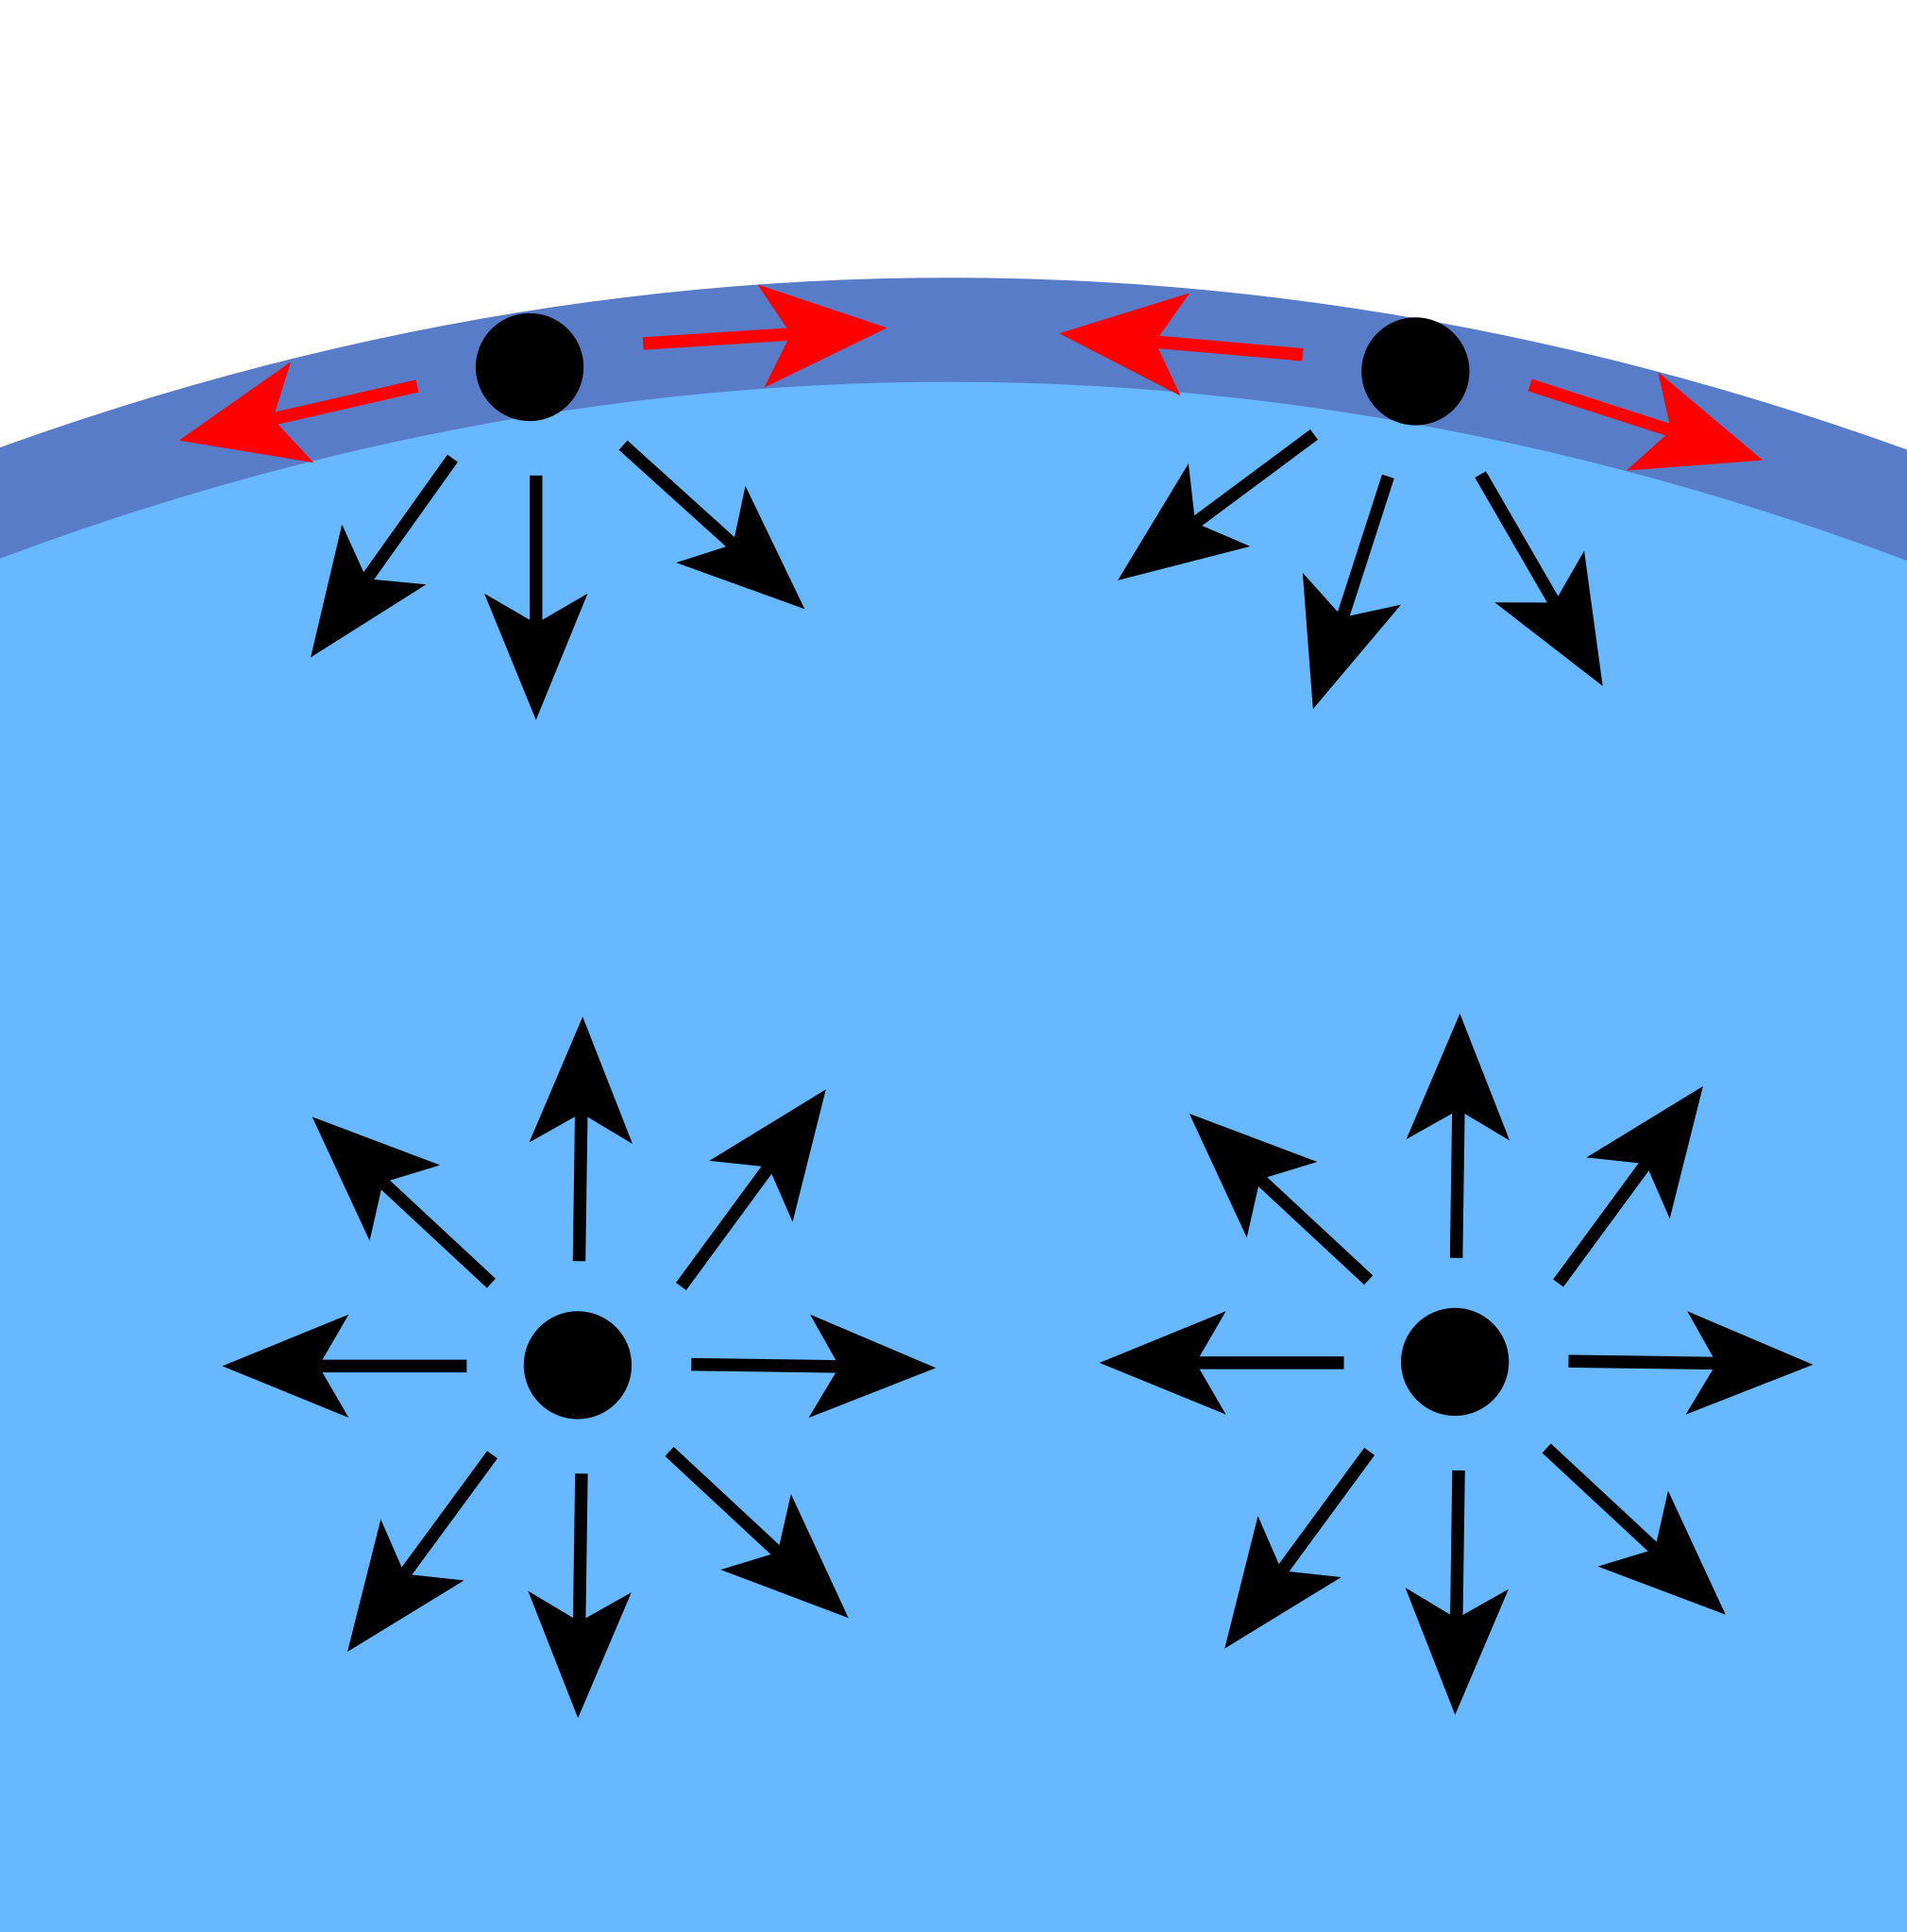
\includegraphics[width=0.35\linewidth]{imagens/ts.png}
	\caption*{Fonte: Wikipedia, disponível em https://shorturl.at/lrAGI}
\label{fig:ts}
\end{figure}

\section{Nomenclatura de hidrocarbonetos}
Assim como qualquer outra substância, todo hidrocarboneto precisa de ao menos dois conjuntos de informação: (a) uma fórmula que caracteriza suas propriedades e (b) um nome que define sua unicidade. Uma vez que são conhecidos centenas de milhares de hidrocarbonetos distintos, torna-se obrigatório o uso de alguma sistematização para criação de nomes únicos.

Esta imensa tarefa está centralizada na entidade conhecida como IUPAC (International Union for Pure and Applied Chemistry, ou União Internacional para Química Pura e Aplicada) e está registrada no chamado "BlueBook", documento específico para nomenclatura de substâncias orgânicas.

Devemos alertar o leitor que, uma vez que são conhecidas milhões de substâncias orgânicas, a quantidade de regras e orientações sugeridas pela IUPAC é relativamente grande e abordaremos neste documento, aos poucos, parte dessas regras, pois nossa obra tem escopo bem definido não necessita de todas as regras. Deixamos aqui a curiosidade do leitor na leitura das regras previstas na versão 3 do BlueBook.

\subsection{Nomenclatura substitutiva}
Este é o principal método utilizado para nomenclatura de substâncias orgânicas e, mais amplamente, para substâncias que possuam elementos dos grupos 13 a 17 da Classificação Periódica dos Elementos. De modo geral, uma substância orgânica tem seu nome construído a partir de regras sistemáticas para que cada nome seja inequívoco, utilizando ao menos dois elementos:

\begin{description}
	\item \textbf{Hidreto pai ou cadeia principal}: é uma substância formada apenas por uma dada cadeia carbônica, sem qualquer grupo funcional, seja com cadeia normal, ramificada, cíclica, aromática ou ainda heteregênea, conforme pode ser observado na figura \ref{fig:hp} a seguir.
	
	\begin{figure}[H]
		\centering
		\caption{Exemplos de hidretos pai}
		\vspace{0.5cm}
		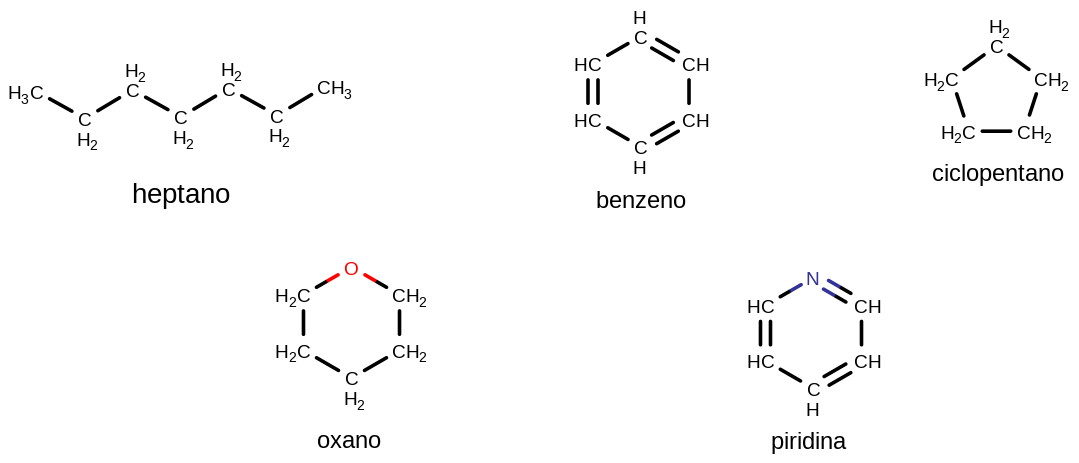
\includegraphics[width=1\linewidth]{imagens/hidretos_pai.png}
	\label{fig:hp}
	\end{figure}

	\item \textbf{Um grupo funcional principal}: caso a substância possua mais de um grupo funcional, um deles é o chamado \textbf{grupo funcional principal}, conforme pode ser visto na tabela \ref{senioridade} a seguir. As colunas "Prefixo" e "Sufixo" indicam, respectivamente, o nome de cada grupo funcional quando este não é a função principal (prefixo) e quando este é a função pricipal (sufixo).
\end{description}

Quando falamos da nomenclatura substitutiva, considere que um átomo de hidrogênio (por exemplo) tenha sido substituído por outro átom o ou grupo de átomos.

\begin{table}[!h]
	%\begin{tabular}
	\begin{center}
	\caption{\label{senioridade}Grupos funcionais em ordem decrescente de senioridade (prioridade)}
	\vspace{0.5cm}
	\begin{tabular}{l c c c}
	\hline
	Função orgânica& Fórmula & Prefixo & Sufixo\\
	\hline
	Carboxilatos & \ce{-COO$^-$} & carboxilato & alcoxicarbonil\\
	Ácido carboxílico & \ce{-COOH} & ácido carboxílico & carboxi\\
	Ésteres & \ce{-COOR} & R-oato & R-oxicarbonil\\
	Haletos de acila & \ce{-COOX} & oil haleto & halocarbonil\\
	Amidas & \ce{-COONH2} & amida & carbamoil\\
	Nitrilas & \ce{-CN} & nitrila & ciano\\
	Aldeídos & \ce{-COH} & al & oxo\\
	Cetonas & \ce{-CO-} & ona & oxo\\
	Álcoois & \ce{-OH} & ol & hidroxi\\
	Tióis & \ce{-SH} & tiol & sulfanil\\
	Aminas & \ce{-NH2} & amina & amino\\
	Iminas & \ce{=NH} & imina & imino\\
	\hline
	\end{tabular}
	\end{center}
\end{table}

\begin{tcolorbox}[colback=blue!5!white,colframe=gray!75!black,title=Atenção!]
	Embora esta seção {\thesection} trate da nomenclatura de hidrocarbonetos, ficam lançadas as bases para a nomenclatura de muitas outras funções orgânicas. Este livro não cobre todas as funções orgânicas conhecidas por tratar-se de de uma obra de caráter básico, e o trabalho de criação das regras de nomenclatura orgânica estende-se há anos a certamente perdurará por outros ainda.
  \end{tcolorbox}




Caso o hidreto pai possua algum grau de insaturação (ligações duplas ou triplas), o sufixo do hidreto se altaera para "eno" ou "ino", indicando as insaturações possível, com os localizadores adequados.

Naturalmente, a presença dos localizadores implica na necessidade da numeração da cadeia carbônica e, como consequência da presença de insaturação ou grupos funcionais, a numeração da cadeia igualmente segue regras bastante rígidas para manter a unicidade de cada nome.

A substância ilustrada abaixo, na figura \ref{fig:46} possui um nome construído pela nomenclatura substitutiva, onde átomos de hidrogênio foram substituídos de um dado hidreto pai.

\begin{figure}[H]
	\centering
	\caption{Exemplo de aplicação da nomenclatura substitutiva.}
	\vspace{0.5cm}
	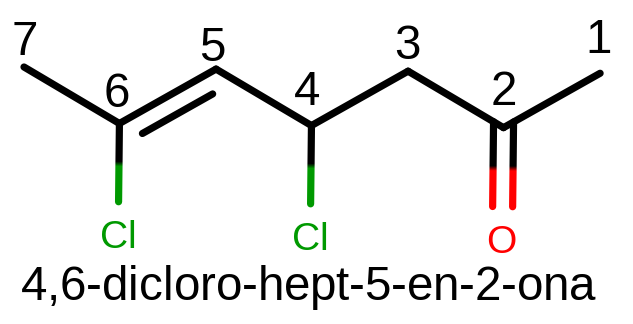
\includegraphics[width=0.6\linewidth]{imagens/46dicloro.png}
\label{fig:46}
\end{figure}

Podemos observar na figura que o hidreto pai consiste em uma cadeia carbônica com 7 átomos, com uma ligação dupla, o que por si só já exige a presença de localizadores, nos obrigando a numerar a cadeia carbônica, restando a dúvida de por onde a iniciar.

A numeração de um hideto pai (ou um copmposto pai, mais genericamente), deve ser efetuada por meio da aplicação dos seginte critérios:

\begin{enumerate}
	\item menor numeração possível para heteroátomos;
	\item menor numeração possível para hidrogênios indicados\footnote{Em determinadas circunstâncias é necessário indicar no nome de um anel, ou sistema de anéis, contendo o número máximo de ligações duplas não cumulativas, uma ou mais posições onde nenhuma ligação múltipla está anexada. Isso é feito especificando a presença de um átomo de hidrogênio 'extra' em tais posições pela citação do local numerado apropriado seguido por um H maiúsculo em itálico};
	\item menor posição possível para o grupo funcional principal;
	\item menor posição para insaturações;
	\item menor posição possível para substituintes indicados por prefixos;
	\item menor posição possível para substituintes em ordem de citação.
\end{enumerate}

Nossa próxima dúvida é a seguinte: por qual extremidade da cadeia com 7 átomos de carbono devemos iniciar a numeração? Consultando os dados presentes na tabela \ref{senioridade}, concluímos que o grupo funcional cetona possui maior senioridade (ou prioridade) na numeração, obedecendo o item 3 logo acima. Assim, a numeração do hidreto pai deve se iniciar na extremidade esquerda da cadeia, o que deixa, automaticamente, a ligação dupla na menor posição possível, restando apenas indicar a posição dos dois grupos funcionais (haleto) com menor prioridade, o que explica inequivocamente o nome da substância da figura \ref{fig:46}.

Analise o próximo exemplo, ilustrado na figura \ref{fig:octadieno} a seguir.

\begin{figure}[H]
	\centering
	\caption{Exemplo de aplicação da nomenclatura substitutiva.}
	\vspace{0.5cm}
	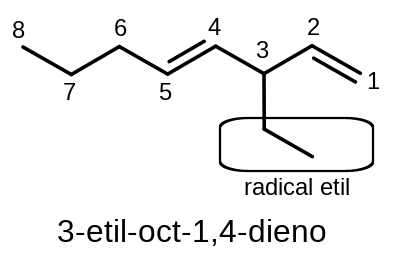
\includegraphics[width=0.6\linewidth]{imagens/octadieno.png}
\label{fig:octadieno}
\end{figure}

Como trata-se de um hidrocarboneto, não há grupos funcioniais na disputa por senioridade, deixando a discussão apenas para decisão entre os radicais substitutintes e as insaturações. Como estas últimas possuem maior senioridade que os radicais, a nmewração da cadeia deve iniciar-se em uma extremidade que deixa as insaturações nas memores posições possíveis da numeração. Finalmene, existe um radical \textbf{etil} conectado ao carbono 3 do hidreto pai. Assim, o nome da substância é \textbf{3-etil-oct-1,4-dieno}. 

Finalizando, convidamos o leitor a examinar a estrutura a seguir, na figura \ref{fig:etenil}, e identificar o número de átomos de carbono do hidreto pai.

\begin{figure}[H]
	\centering
	\caption{Exemplo de aplicação da nomenclatura substitutiva.}
	\vspace{0.5cm}
	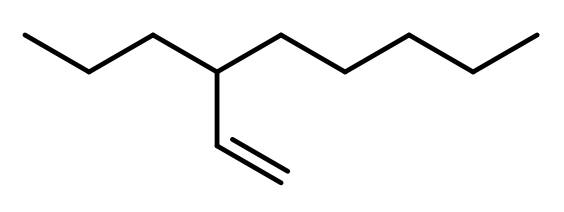
\includegraphics[width=0.6\linewidth]{imagens/etenil.png}
\label{fig:etenil}
\end{figure}

Recomendações da IUPAC anteriores a 2013 sugeriam que o hidreto pai deveria conter eventuais insaturações, mas a recomendação mais atual sugere que o hidreto pai seja aquele com maior número de átomos de carbono, contendo ou não a insaturação. Portanto, o nome da substância da figura \ref{fig:etenil} é mostrado a seguir.

\begin{figure}[H]
	\centering
	\caption{Exemplo de aplicação da nomenclatura substitutiva.}
	\vspace{0.5cm}
	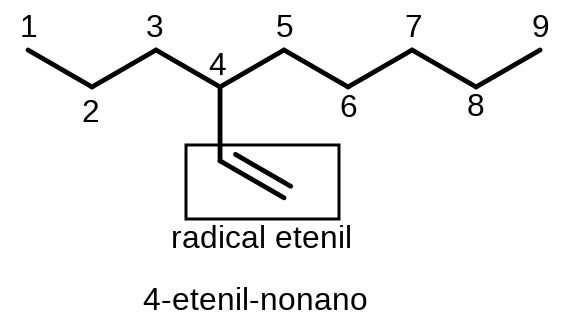
\includegraphics[width=0.6\linewidth]{imagens/nomeetenil.png}
\label{fig:nomeetenil}
\end{figure}